\label{1.3.2}

A morphism whose unerlying map on the topological spaces is a homeomorphism need not be an isomorphism.

\begin{enumerate}[label = (\alph*)]
    \item For example, let $\phi: \A^1 \longrightarrow \A^2$ be defined by $t \mapsto (t^2, t^3)$. Show that $\phi$ defines a bijective bicontinuous morphism on $\A^1$ onto the curve $y^2 = x^3$, but that $\phi$ is not an isomorphism.

    \item For another example, let the characteristic of the base field $k$ be $p > 0$ and define a map $\phi: \A^1 \longrightarrow \A^1$ by $t \mapsto t^p$. Show that $\phi$ is bijective and bicontinuous but not an isomorphism. This is called the \emph{Frobenius morphism}.
\end{enumerate}

\begin{proof}
    \begin{enumerate}[label = (\alph*)]
        \item This map is induced by the algebra homomorphism $k[x, y] \longrightarrow k[t]$ via $x \mapsto t^2$, $y \mapsto t^3$. The image is certainly contained in $V(y^2 - x^3)$. Any $(a, b) \in V(y^2 - x^3)$ is in the image. Indeed, if $a \neq 0$ take $t = \frac{b}{a}$. Else, take $t = 0$. In fact, this defines an inverse to $\phi$, so it is a bijective morphism.

        Next we will show that it is a homeomorphism. Indeed, we will do this by showing hat the subspace topology on $V(y^2 - x^2)$ is the cofinite topology. As the topology on $\A^1$ is also the cofinite topology, this bijection will automatically be a homeomorphism. Indeed, any nonempty closed subset of $V(y^2 - x^3)$ is (uniquely) the finite union of irreducible closed subsets as it is a Noetherian space. Hence, we consider some $F \subseteq V(y^2 - x^3)$ closed and irreducible. If $F < V(y^2 - x^3)$ then we want to show that it is finite. Indeed, if strict inclusion holds then $\dim F < \dim V(y^2 - x^3)$. As the latter has dimension 1 -- for instance because the integral closure of its coordinate ring is $k[t]$ -- $\dim F = 0$. Hence, it is a single point. Thus, any proper closed subset of $V(y^2 - x^3)$ is finite, so its topology is the cofinite one. Hence, the bijection $\phi$ takes proper closed (finite) subsets precisely to proper closed (finite) subsets and it is a homeomorphism.

        Finally, we will show that $\phi$ is not an isomorphism of varieties. These are affine varieties so it suffices to check their coordinate rings. Indeed, on coordinate rings, the map is $k[x, y]/(y^2 - x^3) \longrightarrow k[t]$ via $x \mapsto t^2$, $y \mapsto t^3$. This has image $k[t, t^2] < k[t]$ so it is not an isomorphism. In fact, we can do better. Not only is $\phi$ not an isomorphism, there is no isomorphism between these varieties. Again, it suffices to look at their coordinate rings. $k[t]$ is a UFD but $k[x, y]/(y^2 - x^3) \cong k[t^2, t^3]$ is not. Indeed, $y^2 = x^3$ (and $(t^2)^3 = (t^3)^2$) are distinct irreducible factorizations. Also just for fun, the $k[t^2, t^3]$ is not normal by $k[t]$ is.

        As an aside, that we do not prove in any detail, the inverse map we defined is a rational function away from 0, so this suggests that the difference between these two varieties is at 0. Indeed, look at figure \ref{fig1.3.1} below.

        \begin{figure}[h]
            \centering
            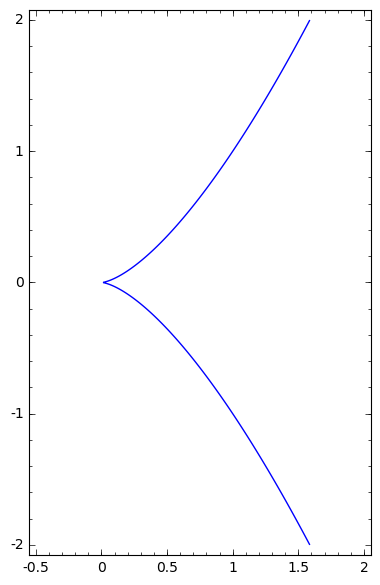
\includegraphics[scale=0.75]{cuspidal-cubic}
            \caption{The cuspidal cubic in $\A^2$}
            \label{fig1.3.1}
        \end{figure}

        Of course this was draw in the real plane, but the point is that there is a cusp at 0, suggesting geometrically what we said above. Also notable is that this variety is sort of ``parametrized" by the affine line, but it lacks ``smoothness" at 0 so this is not an isomorphism. \ref{1.3.17} covers this a bit more.

        \item This map is injective because it is a field homomorphism. It is onto because $k$ is algebraically closed. Indeed, take some $a \in k$. Then the polynomial $t^p - a$ has a root in $k$. As described in part (a), because $\A^1$ has the cofinite topology, this is therefore a homeomorphism. It is given by the algebra homomorphism $k[t] \longrightarrow k[t]$ via $t \mapsto t^p$ so it is a morphism of varieties. Of course, this map has image $k[t^p] < k[t]$, so it is not an isomorphism.
    \end{enumerate}
\end{proof}
